% !TeX program = xelatex
% 第三章 3.2：接在 03_01_kinematics.tex 之後，不另加 chapter。
% 需要 amsmath、amssymb；章節與公式由 LaTeX 自動編號。
% 引用沿用第一章已定義之 grandia2019frequency，不重複新增 BibTeX。

% ==================================================
% 3.2 手臂設定點追蹤與增廣預測模型
% ==================================================
\section{手臂設定點追蹤與增廣預測模型}
\label{sec:arm_augmented_prediction}

前節建立了底盤與手臂的運動學關係，但控制器所產生的命令，仍需經過執行介面與關節位置控制器，才能形成實際運動。Grandia 等人\cite{grandia2019frequency}指出，未建模的致動器動態與頻寬限制，可能影響規劃運動的可執行性。針對本研究採用的手臂位置命令介面，本節建立設定點追蹤模型，並將實際關節位置與位置設定點共同納入預測狀態，使控制器能描述命令至關節運動之間的追蹤關係。

% ==================================================
% 3.2.1 手臂位置命令與伺服追蹤動態
% ==================================================
\subsection{手臂位置命令與伺服追蹤動態}
\label{subsec:arm_setpoint_servo}

令 $s_a\in\mathbb{R}^{6}$ 為手臂關節位置設定點，$u_a\in\mathbb{R}^{6}$ 為其變化率，單位分別為 rad 與 rad/s。執行端將 $u_a$ 積分為位置設定點，再由關節位置控制器追蹤。因此，$u_a$ 描述的是設定點的移動速率，與前節運動學中的實際關節速度 $\dot{q}_a$ 具有不同意義。

以 $\Delta t_p$ 表示物理更新步長，$j$ 表示物理步索引。定義 $q_a^{j}$ 為該步量測的實際關節位置，$s_a^{j}$ 為該步完成寫入後、作用於下一物理區間的位置設定點。依此取樣時序，採用下列逐軸一階仿射模型：
\begin{equation}
    \begin{aligned}
        q_a^{j+1}
        &= (I_6-D_{\alpha})q_a^{j}
           +D_{\alpha}s_a^{j}+b_a, \\
        s_a^{j+1}
        &= s_a^{j}+\Delta t_p u_a^{j},
    \end{aligned}
    \label{eq:ch3_physics_step_arm_model}
\end{equation}
其中 $D_{\alpha}=\operatorname{diag}(\alpha_1,\ldots,\alpha_6)$，$0<\alpha_i<1$ 為第 $i$ 軸的每物理步追蹤係數，$b_a\in\mathbb{R}^{6}$ 為每物理步的偏置項。$u_a^{j}$ 表示此更新關係中的設定點變化率，其對應的設定點增量為 $s_a^{j+1}-s_a^{j}$。第一式描述關節在目前已寫入設定點下的追蹤，第二式則描述下一步設定點的積分更新，兩者的時間索引須與執行端紀錄一致。

若以一階系統解讀其衰減特性，追蹤係數可換算為等效時間常數
\begin{equation}
    \tau_i=-\frac{\Delta t_p}{\ln(1-\alpha_i)},
    \qquad i=1,\ldots,6.
    \label{eq:ch3_arm_equivalent_time_constant}
\end{equation}
當設定點固定且偏置不為零時，第 $i$ 軸的模型穩態偏差為 $(b_a)_i/\alpha_i$。因此，追蹤係數與偏置需共同估計，才能描述設定點與實際關節位置之間的關係。

上述模型描述指定操作條件下的命令追蹤特性，未直接建立馬達力矩、關節慣量或接觸力的動力學。以下先考慮命令已生效，且於一個控制週期內保持固定的情形；命令延遲與在途命令之處理，將於執行動態補償一節另行說明。

% ==================================================
% 3.2.2 實際關節位置與設定點之增廣狀態
% ==================================================
\subsection{實際關節位置與設定點之增廣狀態}
\label{subsec:augmented_arm_state}

控制器更新週期通常與物理更新步長不同。令控制週期為 $\Delta t=m\Delta t_p$，其中 $m$ 為正整數，並以 $k$ 表示控制步索引。在第 $k$ 個控制週期內，令設定點變化率保持為 $u_{a,k}$。由式\eqref{eq:ch3_physics_step_arm_model}反覆代入 $m$ 次，可得控制步的手臂預測模型：
\begin{equation}
    \begin{aligned}
        q_{a,k+1}
        &= A_q q_{a,k}+A_s s_{a,k}
           +B_a u_{a,k}+c_a, \\
        s_{a,k+1}
        &= s_{a,k}+\Delta t u_{a,k}.
    \end{aligned}
    \label{eq:ch3_control_step_arm_model}
\end{equation}
令 $\beta_i=1-\alpha_i$，各軸係數分別為
\begin{equation}
    \begin{aligned}
        A_q
        &=\operatorname{diag}(\beta_1^m,\ldots,\beta_6^m), \\
        A_s
        &=I_6-A_q, \\
        B_a
        &=\operatorname{diag}(g_1,\ldots,g_6), \\
        g_i
        &=\alpha_i\Delta t_p
          \sum_{\ell=0}^{m-1}\ell\,\beta_i^{m-1-\ell}, \\
        (c_a)_i
        &=(b_a)_i\frac{1-\beta_i^m}{\alpha_i},
        \qquad i=1,\ldots,6.
    \end{aligned}
    \label{eq:ch3_arm_composed_coefficients}
\end{equation}
其中 $A_q$ 與 $A_s$ 為無因次矩陣，$B_a$ 具有時間尺度，$c_a$ 為控制週期內累積的偏置。式\eqref{eq:ch3_arm_composed_coefficients}由既定取樣順序推導，因此 $B_a$ 一般不等於 $\Delta t I_6$。即使 $u_{a,k}=\mathbf{0}$，只要實際關節位置與設定點之間仍有差異，關節仍可能繼續朝設定點移動。

為與底盤幾何誤差模型整合，定義增廣狀態與控制輸入為
\begin{equation}
    \zeta_k=
    \begin{bmatrix}
        e_{B,k} \\
        q_{a,k} \\
        s_{a,k}
    \end{bmatrix}
    \in\mathbb{R}^{15},
    \qquad
    u_k=
    \begin{bmatrix}
        \delta\xi_k \\
        u_{a,k}
    \end{bmatrix}
    \in\mathbb{R}^{9},
    \label{eq:ch3_augmented_state_input}
\end{equation}
其中 $e_{B,k}$ 與 $\delta\xi_k$ 沿用前節定義，實際底盤速度命令為 $\xi_{r,k}+\delta\xi_k$。六維設定點為執行模型的內部狀態，其增廣不改變機器人的九個運動自由度，也不增加控制輸入維度。

結合式\eqref{eq:ch3_discrete_base_error_model}與式\eqref{eq:ch3_control_step_arm_model}，得到全身增廣預測模型
\begin{equation}
    \zeta_{k+1}=F_k\zeta_k+G u_k+d,
    \label{eq:ch3_augmented_prediction_dynamics}
\end{equation}
其中
\begin{equation}
    F_k=
    \begin{bmatrix}
        A_{B,k} & \mathbf{0}_{3\times6} & \mathbf{0}_{3\times6} \\
        \mathbf{0}_{6\times3} & A_q & A_s \\
        \mathbf{0}_{6\times3} & \mathbf{0}_{6\times6} & I_6
    \end{bmatrix}
    \in\mathbb{R}^{15\times15},
    \label{eq:ch3_augmented_state_matrix}
\end{equation}
\begin{equation}
    G=
    \begin{bmatrix}
        B_B & \mathbf{0}_{3\times6} \\
        \mathbf{0}_{6\times3} & B_a \\
        \mathbf{0}_{6\times3} & \Delta t I_6
    \end{bmatrix},
    \qquad
    d=
    \begin{bmatrix}
        \mathbf{0}_{3} \\
        c_a \\
        \mathbf{0}_{6}
    \end{bmatrix},
    \label{eq:ch3_augmented_input_bias}
\end{equation}
且 $G\in\mathbb{R}^{15\times9}$、$d\in\mathbb{R}^{15}$。在追蹤係數與偏置固定時，手臂區塊為仿射模型；底盤區塊則保留前節的局部一階近似。

末端位姿仍由底盤位姿與實際關節位置決定。於預測時刻，先由幾何誤差還原底盤位姿，再依式\eqref{eq:ch3_wholebody_forward_kinematics}計算末端位姿：
\begin{equation}
    \begin{aligned}
        X_{B,k}
        &=X_{r,k}\exp\!\left(\widehat{e}_{B,k}\right), \\
        {}^{W}T_{E,k}
        &={}^{W}T_B(X_{B,k})\,{}^{B}T_A\,
          {}^{A}T_E(q_{a,k}).
    \end{aligned}
    \label{eq:ch3_augmented_tcp_reconstruction}
\end{equation}
其中 ${}^{W}T_B(X_{B,k})$ 為平面位姿的三維嵌入。位置設定點 $s_{a,k}$ 經由追蹤模型影響後續的 $q_{a,k}$，不直接代入正向運動學。雖然底盤與手臂的狀態轉移以分塊形式表示，兩者仍透過共同的末端目標形成控制耦合，相關目標函數於下一節建立。

位置設定點與實際關節位置的追蹤關係如\cref{fig:ch3_arm_setpoint_tracking}所示。圖中以單軸一階追蹤模型呈現設定點固定後，實際關節仍逐步接近設定點的情形，說明預測時需分別保留實際關節位置 $q_a$ 與位置設定點 $s_a$。

\begin{figure}[htbp]
    \centering
    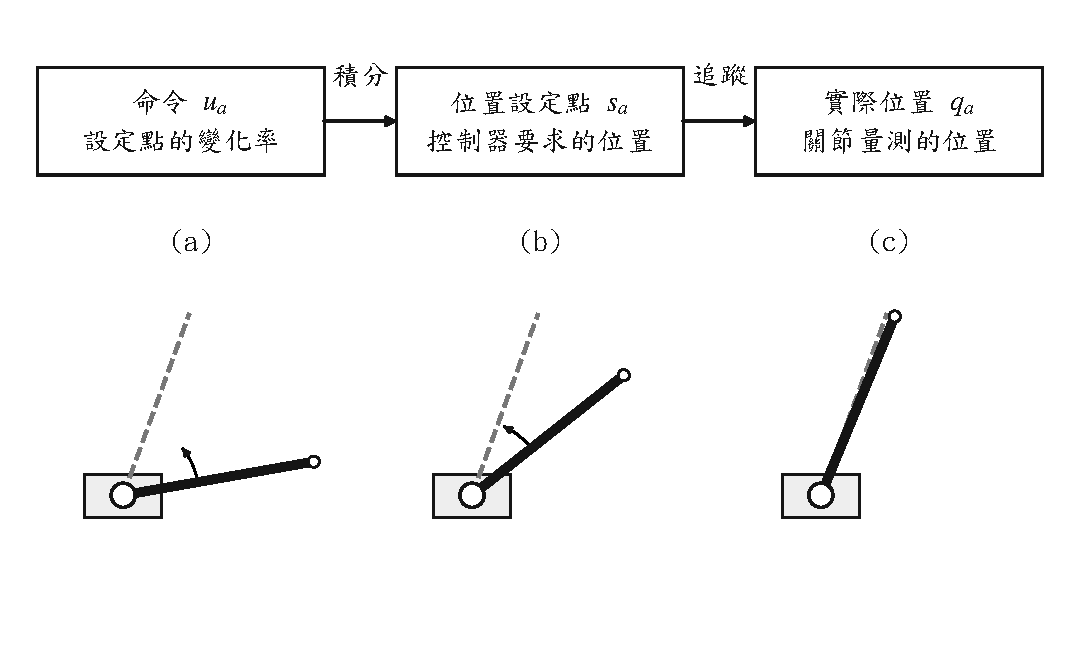
\includegraphics[width=0.98\textwidth]{figsrc/ch03/arm_setpoint_tracking.pdf}
    \caption{手臂設定點與實際關節位置之追蹤關係：(a) 設定點固定；(b) 關節持續追蹤；(c) 關節逐漸接近設定點。虛線與實線分別表示位置設定點與實際關節位置。}
    \label{fig:ch3_arm_setpoint_tracking}
\end{figure}

% ==================================================
% 3.2.3 多步預測模型建立與參數辨識
% ==================================================
\subsection{多步預測模型建立與參數辨識}
\label{subsec:multistep_prediction_identification}

令 $N$ 為預測步數，$i|k$ 表示在第 $k$ 個控制週期，對未來第 $i$ 步的預測。預測初始狀態 $\zeta_{0|k}$ 由對齊至相同取樣時刻的底盤位姿、實際關節位置及執行端設定點建立。設定點須使用執行端回報值，不能在每次求解時直接以實測關節位置取代，否則將消除模型欲描述的追蹤落後。

有限時域內的狀態依下式遞推：
\begin{equation}
    \zeta_{i+1|k}
    =F_{k+i}\zeta_{i|k}+G u_{i|k}+d,
    \qquad i=0,\ldots,N-1.
    \label{eq:ch3_horizon_state_recursion}
\end{equation}
將未來狀態與輸入堆疊為
\begin{equation}
    \mathbf{Z}_k=
    \begin{bmatrix}
        \zeta_{1|k} \\ \vdots \\ \zeta_{N|k}
    \end{bmatrix},
    \qquad
    \mathbf{U}_k=
    \begin{bmatrix}
        u_{0|k} \\ \vdots \\ u_{N-1|k}
    \end{bmatrix},
    \label{eq:ch3_horizon_state_input_stack}
\end{equation}
則可整理為
\begin{equation}
    \mathbf{Z}_k
    =\Phi_k\zeta_{0|k}+\Gamma_k\mathbf{U}_k+\eta_k,
    \label{eq:ch3_condensed_augmented_prediction}
\end{equation}
其中 $\Phi_k\in\mathbb{R}^{15N\times15}$ 為初始狀態傳遞矩陣，$\Gamma_k\in\mathbb{R}^{15N\times9N}$ 為輸入影響矩陣，$\eta_k\in\mathbb{R}^{15N}$ 為偏置累積向量。各預測步的係數可由式\eqref{eq:ch3_horizon_state_recursion}依序建立；$\Gamma_k$ 具有分塊下三角結構，表示未來命令僅影響其作用後的預測狀態。此形式可將預測關節位置、設定點與底盤誤差表示為控制序列的仿射函數，供後續目標函數與限制條件使用。

手臂模型參數由設定點與實際關節位置紀錄逐軸辨識。對第 $r$ 個關節，依相同物理步長及取樣順序形成資料對，定義關節位移 $\Delta q_r^{j}=q_r^{j+1}-q_r^{j}$ 與追蹤差 $\varepsilon_r^{j}=s_r^{j}-q_r^{j}$，並以最小平方法估計參數：
\begin{equation}
    \begin{aligned}
        J_r(\alpha_r,b_r)
        &=\sum_{j\in\mathcal{I}_{\mathrm{est}}}
          \left(\Delta q_r^{j}-\alpha_r\varepsilon_r^{j}-b_r\right)^2, \\
        (\hat{\alpha}_r,\hat{b}_r)
        &=\underset{\alpha_r,b_r}{\operatorname{arg\,min}}\;
          J_r(\alpha_r,b_r).
    \end{aligned}
    \label{eq:ch3_arm_parameter_identification}
\end{equation}
其中 $\mathcal{I}_{\mathrm{est}}$ 為參數估計資料的索引集合，$q_r^{j}$ 與 $s_r^{j}$ 分別為 $q_a^{j}$ 與 $s_a^{j}$ 的第 $r$ 個分量。估計後檢查 $0<\hat{\alpha}_r<1$，並以未參與估計的資料檢查單步與多步預測誤差。資料依時間先後區分為估計與驗證區段；多步驗證亦須區分是否使用已記錄的後續設定點或命令，避免將事後重播誤差視為線上預測效能。

本研究以既有模擬紀錄建立初始模型參數，辨識設定、預測誤差及適用範圍於第四章說明。透過上述增廣模型，後續控制問題可同時考量實際關節位置與位置設定點，並保留兩者在追蹤動態及運動限制上的差異。
